\documentclass{compiladores}
\usepackage{subcaption}

\usepackage{tikz}
\usepackage{qtree}
\usetikzlibrary{shadows,trees}
\usetikzlibrary{positioning,shadows,arrows,trees,shapes,fit}
\usetikzlibrary{graphs}

\renewcommand{\flecha}{$\rightarrow$}
\newcommand{\vazio}{{\LARGE$\epsilon$}\xspace}

\begin{document}

\begin{center}
{\LARGE Material de Apoio \#69} \\
{\bf Esquemas de tradução para arranjos}
\end{center}

\section{Formulação}

A definição do endereço dentro de um arranjo depende da organização
adotada na linguagem de programação: se é por linha, coluna ou por
vetor de acesso. No que segue, adotamos a organização {\bf por linha}.
O cálculo do endereço de uma determinada célula de um arranjo
multidimensional é feita de maneira recursiva. Por fins de otimização,
podemos dividir o cálculo em duas partes: na declaração e no acesso.

Na declaração, todas as informações a respeito do endereçamento são
conhecidas (quantas dimensões, tamanho e limite de cada dimensão),
permitindo a definição de uma constante $C_A$ que é registrada na
entrada da tabela de símbolos para o identificador do arranjo.  Seja
$A[low_0..high_0][low_1..high_1]..[low_k..high_k]$ os limites das
dimensões, \emph{base} o endereço de base do arranjo (de acordo com a
posição de sua declaração e dependendo do escopo), e \emph{w} o
tamanho do elemento deste vetor (relacionado ao tipo), o cálculo do
valor constante $C_A$ de um arranjo $A$ é dado pelo seguinte:
\begin{equation}
C_A = base - r_k * w
\end{equation}
\begin{equation}
r_k = \left\{ 
\begin{array}{l l}
low_k & \quad \text{se $k = 0$} \\
r_{k-1} * |high_k-low_k| + low_k & \quad \text{se $k \geq 1$}
\end{array} \right.
\end{equation}

No acesso, as informações dos índices (identificando unicamente uma
célula) estão disponíveis. Os índices podem eventualmente ser
calculados a partir de expressões aritméticas. Seja
$A[i_0][i_1]..[i_k]$ os índices, o cálculo do endereço final é dado
pelo seguinte ($w$ é o tamanho do elemento, $C_A$ foi calculado na
declaração):

\begin{equation}
endereco = C_A + d_k * w
\end{equation}
\begin{equation}
d_k = \left\{ 
\begin{array}{l l}
i_k & \quad \text{se $k = 0$} \\
d_{k-1} * |high_k-low_k| + i_k & \quad \text{se $k \geq 1$}
\end{array} \right.
\end{equation}

\section{Esquemas de tradução}

O conjunto de instruções ILOC é utilizado quando necessário.

Para a {\bf declaração} do arranjo (e cálculo do $C_A$), temos o seguinte esquema:

\begin{tabular}{llll}
 D & \flecha & N$_1$ .. N$_2$ & \{ \et{D.low = N$_1$.val; D.high = N$_2$.val; D.n = mod(D.high - D.low);} \} \\
 L & \flecha & D              & \{ \et{L.r = D.low; L.dim = 0; def\_dim\_size(L.dim, D.high, D.low);} \}\\
 L & \flecha & L$_1$ D        & \{ \et{L.r = L$_1$.r * D.n + D.low; L.dim++; def\_dim\_size (L.dim, D.high, D.low);} \} \\
 DECL & \flecha & T {\bf ident} {\bf [} L {\bf ]} & \{ \et{$C_A$ = base - L.r * T.w; decl(ident, T.type, T.w, $C_A$, get\_dim\_sizes());} \} \\
\end{tabular}

Para o {\bf acesso} de um arranjo (supondo declaração dentro de
uma função -- por isso \et{fp}), temos o seguinte esquema:

\begin{tabular}{llll}
 L & \flecha & D        & \{ \et{L.dim = 0; L.code = D.code; L.d = D.temp;} \} \\
 L & \flecha & L$_1$, D & \{ \et{L.d = temp();
    L.dim = L$_1$.dim+1;
    n = get\_dim\_size (ident, L.dim); x = temp();} \\
   &         &          & \et{L.code = L$_1$.code || D.code || ``mult
     $L_1$.d,  n => x'' || ``add
    x, D.temp => L.d'';}
 \} \\
 ACES & \flecha & {\bf ident [} L {\bf ]} & \{ \et{x=temp();
   ACES.temp=temp();} \\
      &         & & \et{ACES.code = L.code || ``mult w, L.d => x'' ||
        ``add $C_A$, x => y'' ||}  \\
      &         & & \et{``loadAO fp, y => ACES.temp''}; \} \\
\end{tabular}


\section{Um exemplo de uso de declaração}

Para uma declaração de arranjo:
\begin{center}
\et{int cubo[3..5][-2..3][-4..10];}
\end{center}
obtemos um valor de $C_A$ de 178, conformo Figura~\ref{69-fig1}.

\begin{figure}[!htb]
  \centering
  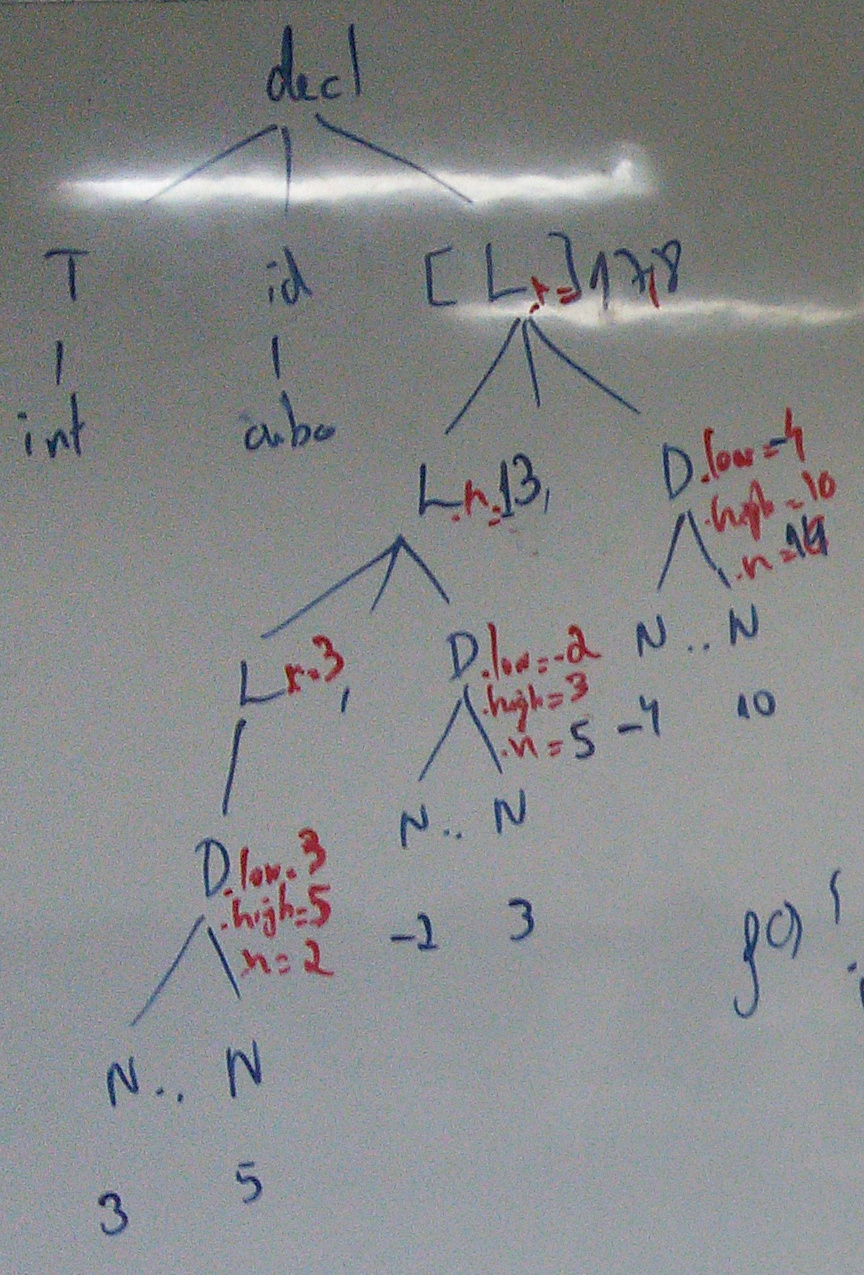
\includegraphics[width=.5\linewidth]{img/69-1.jpg}
  \caption{Solução do exemplo de uso.}
  \label{69-fig1}
\end{figure}


\end{document}